\sectionframe{Stückweise definierte Funktionen}
\subsection{Treppenfunktionen}
\begin{frame}
 \frametitle{Beispiel: Lewig Xanxi}
 \begin{figure}
  \centering
  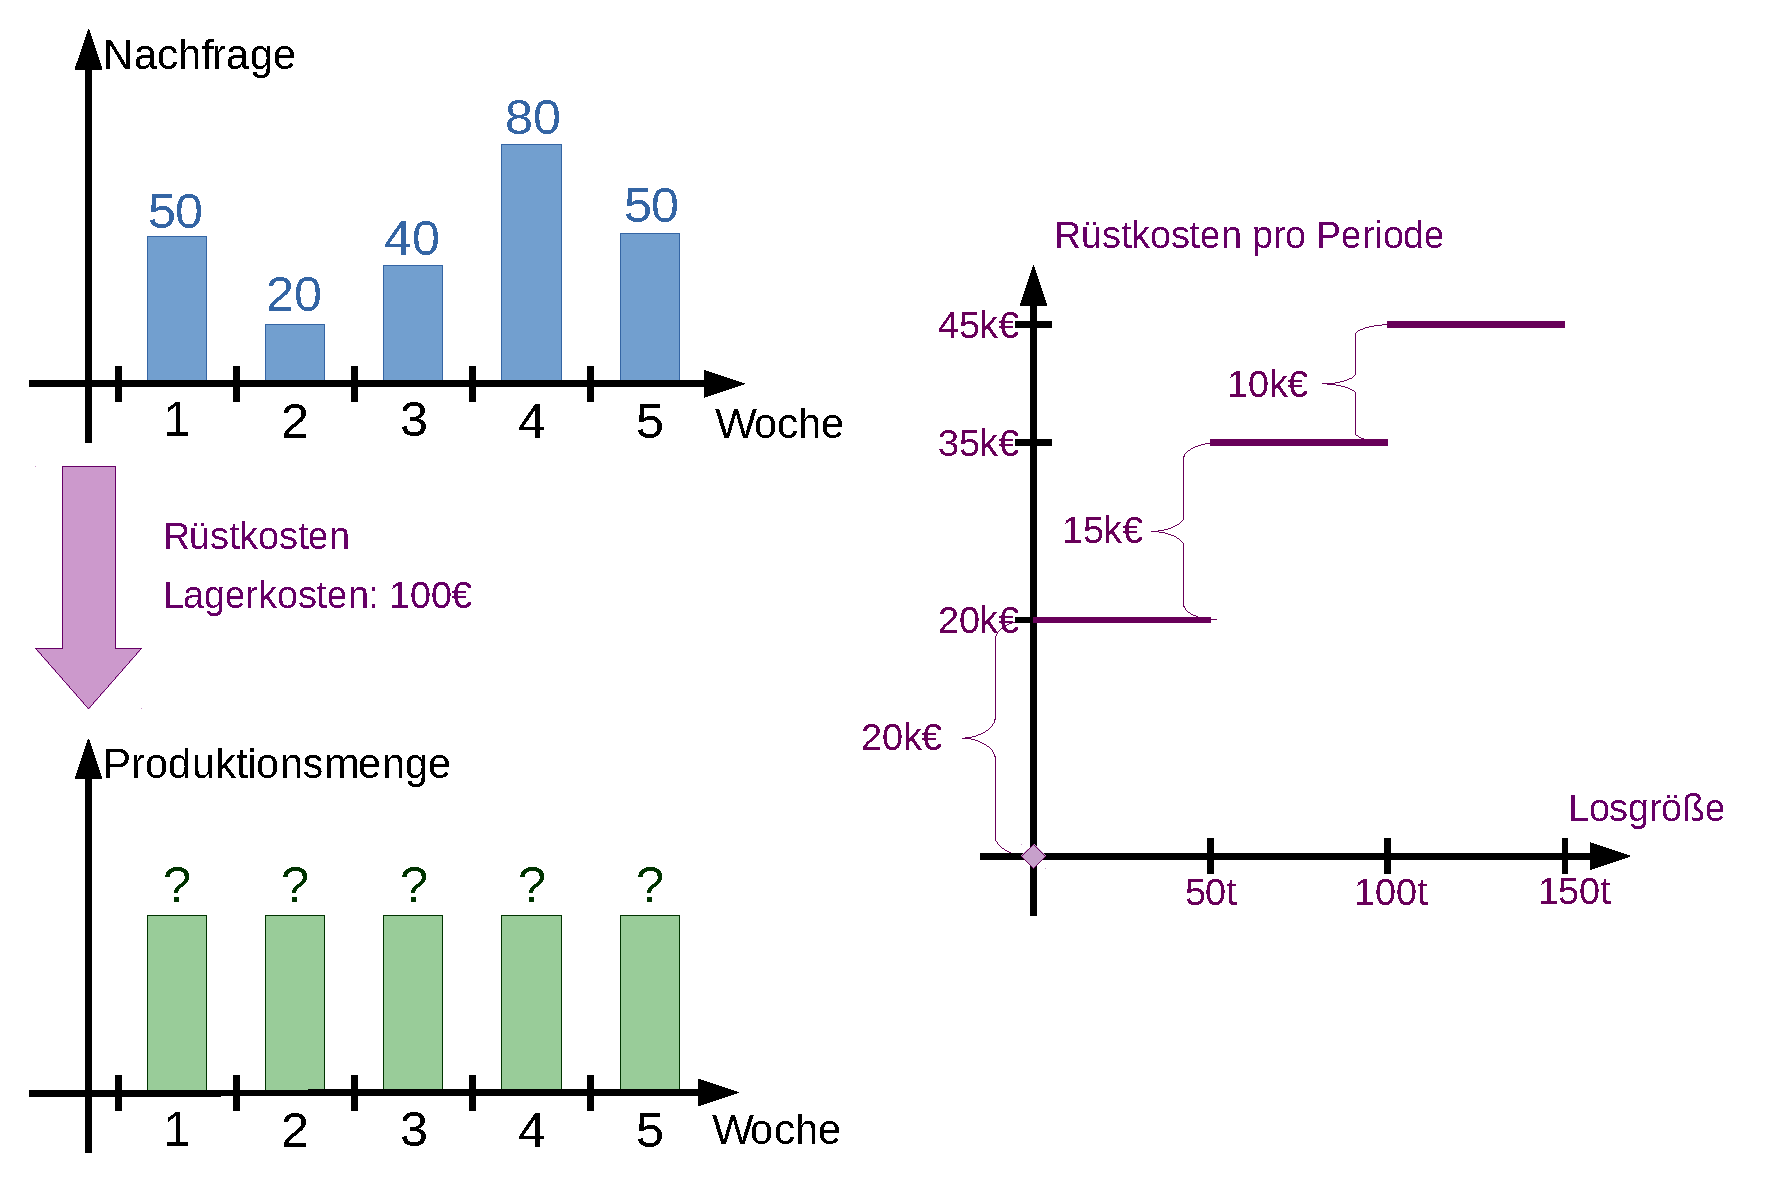
\includegraphics[width=\linewidth]{Bilder/WagnerWhitinProblem2}
 \end{figure}
\end{frame}

\begin{frame}
 \frametitle{Treppenfunktionen}
 \small Sei $x$ eine kontinuierliche Entscheidungsvariable:
 
 \includegraphics<1>[width=\textwidth,page=1]{Bilder/Treppenfunktion}
 \includegraphics<2>[width=\textwidth,page=2]{Bilder/Treppenfunktion}
 \includegraphics<3>[width=\textwidth,page=3]{Bilder/Treppenfunktion}
 \begin{itemize}
  \item<3> z.B.: \structure{$x=\frac{1}{3}\cdot p_1 + \frac{2}{3}\cdot p_2$}
 \end{itemize}
\end{frame}

\begin{frame}
 \frametitle{Entscheidungsvariablen als Konvexkombination der Stützstellen}
 \vspace{-5ex}
 \begin{flushright}
  \includegraphics[width=.5\textwidth,page=3]{Bilder/Treppenfunktion}
 \end{flushright}
 \vspace{-5ex}
 \begin{align*}
  &x = \sum_{n=0}^{N} z_n\cdot p_n\\
  &\sum_{n=0}^N z_n = 1\\
  &0 \leq z_n \leq 1\quad\forall n\in\{1, \ldots, N\}
 \end{align*}
\end{frame}

\begin{frame}
 \frametitle{Auswahl des korrekten Intervalls}
 \begin{flushright}
  \includegraphics[width=.5\textwidth,page=3]{Bilder/Treppenfunktion}
 \end{flushright}
 \vspace{-5ex}
 \begin{align*}
  &\sum_{n=1}^{N}{y_n} = 1\\
  &z_0 \leq y_1\\
  &z_n \leq y_n + y_{n+1}\quad\forall n\in\{1, \ldots, N-1\}\\
  &z_N \leq y_N\\
 \end{align*}
\end{frame}

\begin{frame}
 \frametitle{Vollständige Modellierung}
 \begin{flushright}
  \includegraphics[width=.5\textwidth,page=3]{Bilder/Treppenfunktion}
 \end{flushright}
 \vspace{-15ex}\small
 \begin{align*}
  &f(x) = \sum_{n=1}^N y_n\cdot k_n\\
  &x = \sum_{n=0}^{N} z_n\cdot p_n\\
  &\sum_{n=0}^N z_n = 1\\
  &0 \leq z_n \leq 1\quad\forall n\in\{1, \ldots, N\}\\
  &\sum_{n=1}^{N}{y_n} = 1\\
  &z_0 \leq y_1\\
  &z_n \leq y_n + y_{n+1}\quad\forall n\in\{1, \ldots, N-1\}\qquad\qquad\qquad\mbox{}\\
  &z_N \leq y_N\\
 \end{align*}
\end{frame}


\subsection{Stückweise lineare Funktionen}
\begin{frame}
 \frametitle{Stückweise lineare Funktionen}
 \begin{figure}
  \centering
  \includegraphics<1>[width=\linewidth,page=1]{Bilder/StueckweiseLineareFunktion1}
  \includegraphics<2>[width=\linewidth,page=2]{Bilder/StueckweiseLineareFunktion1}
 \end{figure}
\end{frame}

\begin{frame}
 \frametitle{Funktionswerte als Konvexkombination}
 \begin{flushright}
  \includegraphics[width=.5\textwidth,page=2]{Bilder/StueckweiseLineareFunktion1}
 \end{flushright}
 \vspace{-5ex}
 \begin{align*}
  &x = \sum_{n=0}^{N} z_n\cdot p_n\\
  &\alert{f(x)} = \sum_{n=0}^{N} z_n\cdot \alert{f(p_n)}\\
  &\sum_{n=0}^N z_n = 1\\
  &0 \leq z_n \leq 1\quad\forall n\in\{1, \ldots, N\}\qquad\qquad\mbox{}
 \end{align*}
\end{frame}

\begin{frame}
 \frametitle{Vollständige Modellierung}
 \begin{flushright}
  \includegraphics[width=.5\textwidth,page=2]{Bilder/StueckweiseLineareFunktion1}
 \end{flushright}
 \vspace{-15ex}\small
 \begin{align*}
  &f(x) = \sum_{n=0}^N z_n\cdot k_n\\
  &x = \sum_{n=0}^{N} z_n\cdot p_n\\
  &\sum_{n=0}^N z_n = 1\\
  &0 \leq z_n \leq 1\quad\forall n\in\{1, \ldots, N\}\\
  &\sum_{n=1}^{N}{y_n} = 1\\
  &z_0 \leq y_1\\
  &z_n \leq y_n + y_{n+1}\quad\forall n\in\{1, \ldots, N-1\}\qquad\qquad\qquad\mbox{}\\
  &z_N \leq y_N\\
 \end{align*}
\end{frame}

\subsection{OPL: Der \texttt{piecewise}-Befehl}
\begin{frame}
 \frametitle{Stückweise lineare Funktionen nach Steigung}
 \begin{figure}
  \centering
  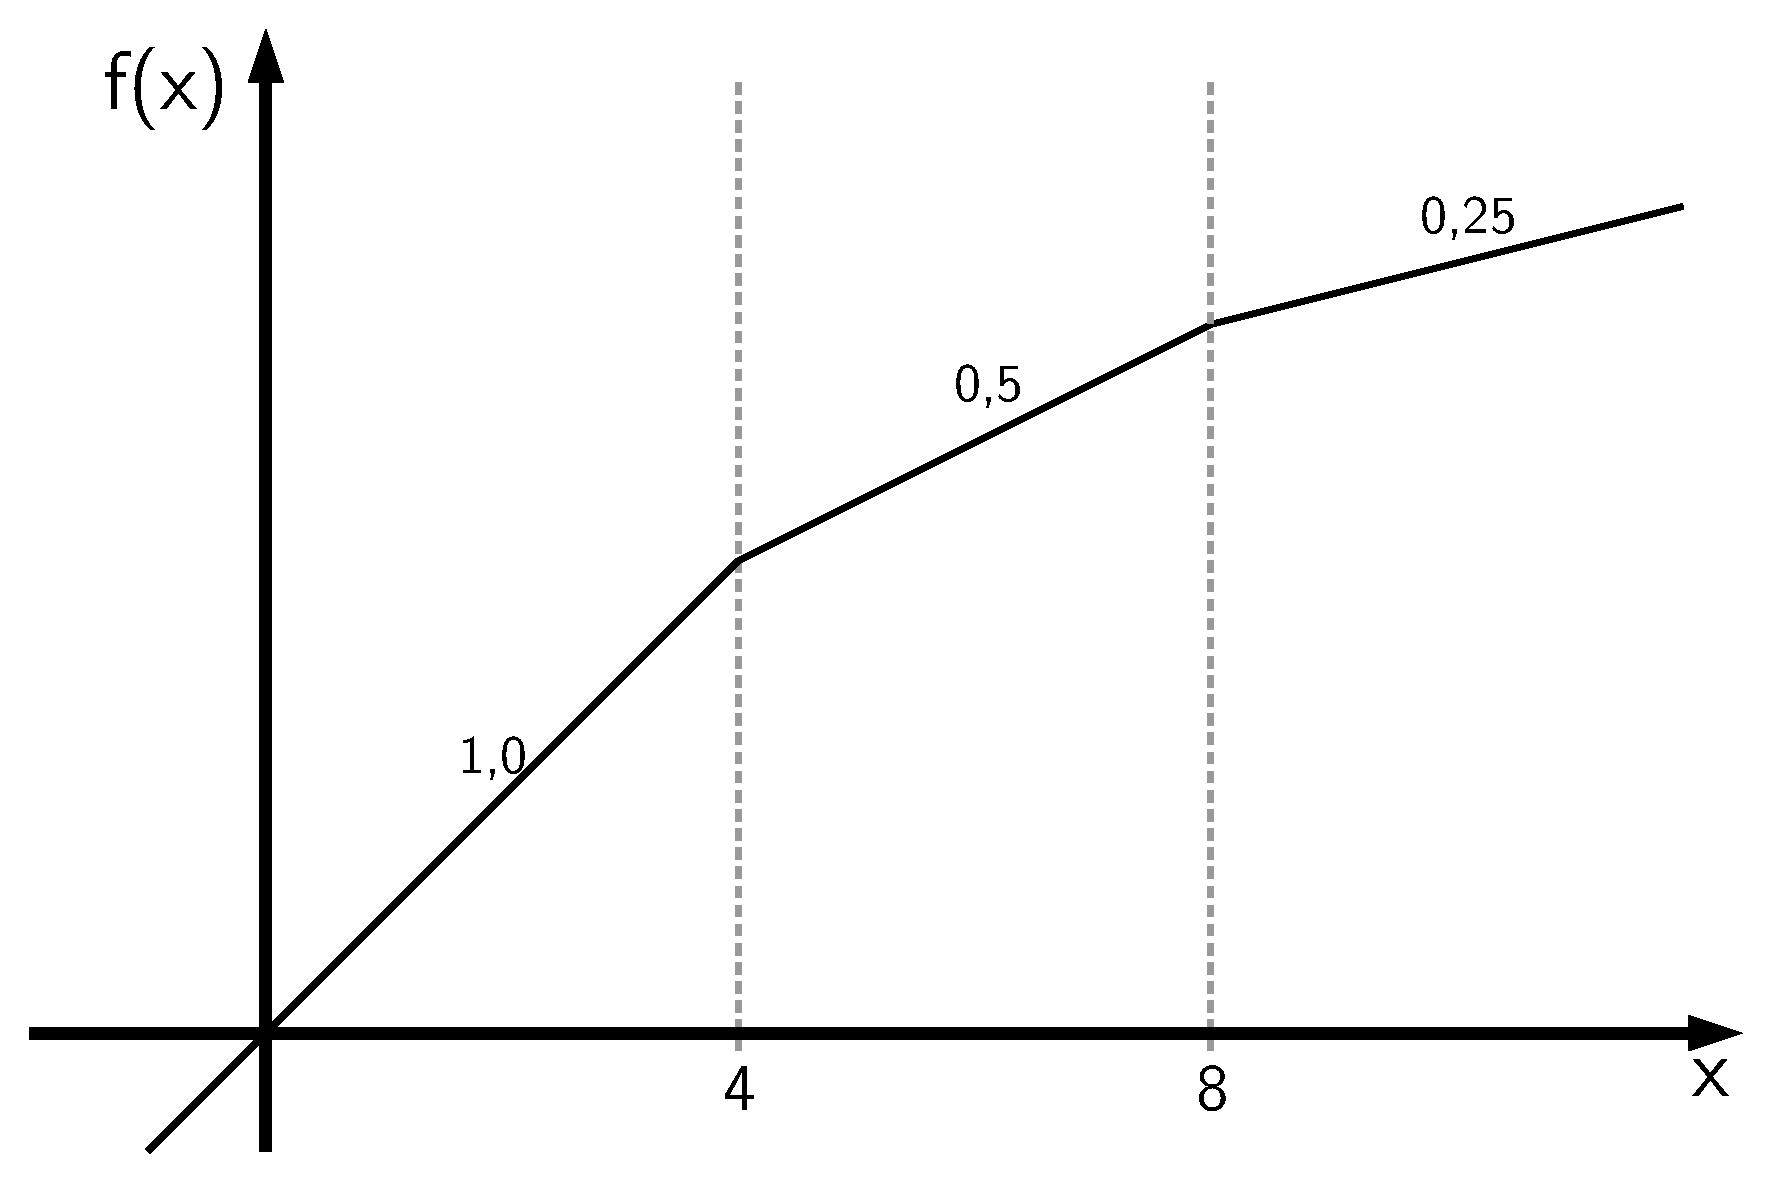
\includegraphics[width=\linewidth,page=1]{Bilder/StueckweiseLineareFunktion3}
 \end{figure}
\end{frame}

\begin{frame}
 \frametitle{Verankerung von stückweise linearen Funktionen}
 \begin{figure}
  \centering
  \includegraphics[width=\linewidth,page=2]{Bilder/StueckweiseLineareFunktion3}
 \end{figure}
\end{frame}

\begin{frame}
 \frametitle{Syntax des \texttt{piecewise}-Befehls}
 Array \texttt{p} der Stützstellen und Array \texttt{s} der Steigungen:
 \begin{center}
  \begin{minipage}{.5\linewidth}
   \ttfamily
    piecewise(i in 1..N)\{\\
    \mbox{}\quad s[i] -> p[i];\\
    \mbox{}\quad s[N+1]\\
    \} (\textsf{\slshape Ankerpunkt}) x;\\
  \end{minipage}
 \end{center}
 \vspace{-3ex}
 \begin{block}{Beispiel aus obiger Abbildung}\ttfamily\footnotesize
  int N = 2;\\
  float p[1..N] = [4, 8];\\
  float s[1..N+1] = [1.0, 0.5, 0.25];\\
  dvar float+ x;\\[2ex]  
  piecewise(i in 1..N)\{\\
    \quad s[i] -> p[i];\\
    \quad s[N+1]\\
  \} (2, 2) x;\\
 \end{block}
\end{frame}

\begin{frame}
 \frametitle{Treppenfunktionen und allgemeine Unstetigkeiten}
 \begin{figure}
  \centering
  \includegraphics[width=\linewidth,page=3]{Bilder/StueckweiseLineareFunktion3}
 \end{figure}
\end{frame}

\begin{frame}
 \frametitle{Treppenfunktionen und allgemeine Unstetigkeiten}
 Zweiter Steigungswert an einem Punkt im \texttt{piecewise}-Befehl wird zu Sprungwert.
 \begin{block}{Beispiel aus obiger Abbildung}\ttfamily\footnotesize
  int N = 3;\\
  float p[1..N] = [4, \alert{4}, 8];\\
  float s[1..N+1] = [1.0, \alert{2.0}, 0.0, 0.5];\\
  dvar float+ x;\\[2ex]  
  piecewise(i in 1..N)\{\\
    \quad s[i] -> p[i];\\
    \quad s[N+1]\\
  \} x;\\
 \end{block}
\end{frame}
